\newcommand{\psd}[1]{{\small\sffamily{\color{blue!60}#1}}}





In the 2D problem above seismic sources was supplied on the border, in
the current one the source is more realistic and comes from a double
couple (point Dirichlet condition). The double couple boundary condition
is a way to impose moments caused by faults that create earthquakes,
here in this problem double couple is imposed using displacement based.

\begin{lstlisting}[style=BashInputStyle]
PSD_PreProcess -dimension 2 -problem soildynamics  -timediscretization newmark_beta \
-useGFP -doublecouple displacement_based -postprocess uav
\end{lstlisting}

Once the step above has been performed, we solve the problem using two
MPI processes, with the given mesh file \psd{soil-dc.msh}.

\begin{lstlisting}[style=BashInputStyle]
PSD_Solve -np 2 Main.edp -v 1 -ns -nw -mesh ./../Meshes/2D/soil-dc.msh
\end{lstlisting}

\begin{figure}[h!]
\centering
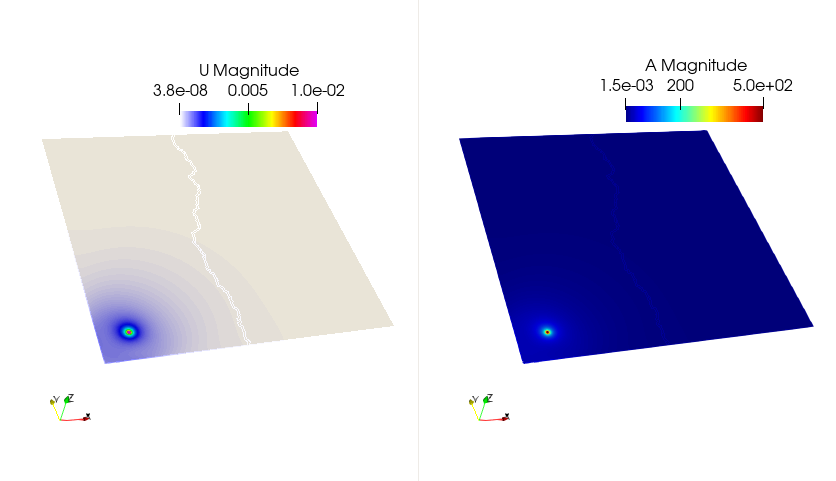
\includegraphics[width=0.45\textwidth]{./Images/sd-2ddcu0.png}
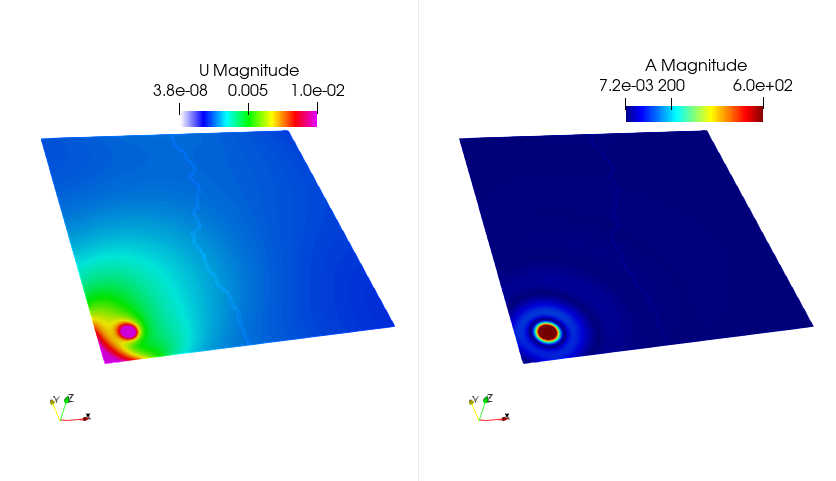
\includegraphics[width=0.45\textwidth]{./Images/sd-2ddcu1.png}\\
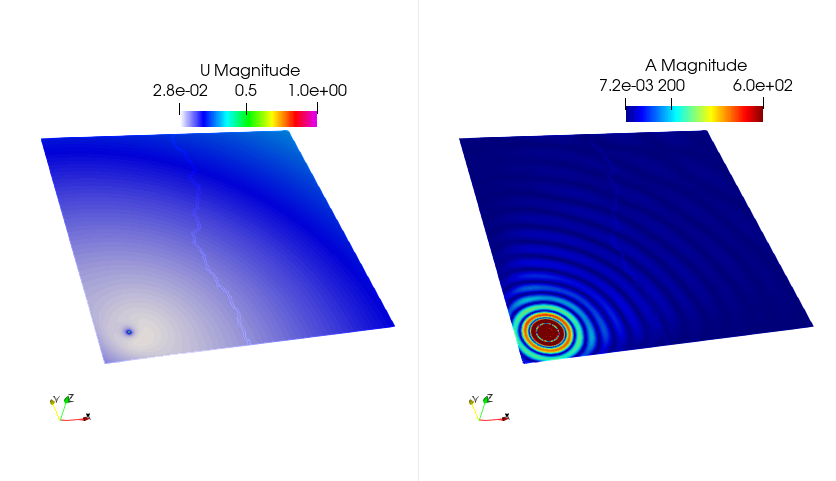
\includegraphics[width=0.45\textwidth]{./Images/sd-2ddcu2.png}
\caption{Finite element displacement and acceleration fields visualized for the 2D problem with ParaView at different timesteps. \label{bar2ddc-sd}}
\end{figure}

Using ParaView for postprocessing the results that are provided in the
\psd{VTUs...} folder, results such as those shown in
figure\textasciitilde{}\ref{bar2ddc-sd} can be extracted.

Similarly try out the 3D problem. However take note that a the mesh
\psd{./../Meshes/2D/soil-dc.msh} is not provided, so you will have to
create your own mesh.
